\documentclass[11pt]{amsart} 
\usepackage{fullpage}

\usepackage{graphicx}

\usepackage{amsmath,amsthm,amssymb}
\usepackage{xcolor}
\usepackage{url}
\usepackage{ mathrsfs }
\newcommand{\ncr}[1]{{\color{blue}\textsf{[[NCR: #1]]}}}

\newcommand     {\abs}[1]       {{\left\lvert{#1}\right\rvert}}



\newcommand{\eff}{\textrm{eff}}
\newcommand{\std}{\textrm{std}}
\newcommand{\sym}{\textrm{sym}}
\newcommand{\SO}{\textrm{SO}}

% important rings
\newcommand{\R}{\ensuremath{\mathbf{R}}}
\newcommand{\C}{\ensuremath{\mathbf{C}}}
\newcommand{\Q}{\ensuremath{\mathbf{Q}}}

\newcommand{\N}{\ensuremath{\mathbf{N}}}
\newcommand{\Z}{\ensuremath{\mathbf{Z}}}
\newcommand{\A}{\ensuremath{\mathbf{A}}}


\newcommand{\ep}{\epsilon}

\newcommand{\D}{\mathcal D_f}
\newcommand{\F}{\ensuremath{\mathcal{F}}}
\newcommand{\E}{\mathcal E_f}


\newcommand\be{\begin{equation}}
\newcommand\ee{\end{equation}}
\newcommand\bi{\begin{itemize}}
\newcommand\ei{\end{itemize}}
\newcommand\ben{\begin{enumerate}}
\newcommand\een{\end{enumerate}}

\newtheorem{fact}{Fact}
\newtheorem{lemma}{Lemma}
\newtheorem{theorem}[lemma]{Theorem}
\newtheorem{defn}[lemma]{Definition}
\newtheorem{assumption}[lemma]{Assumption}
\newtheorem{corollary}[lemma]{Corollary}
\newtheorem{prop}[lemma]{Proposition}
\newtheorem{exercise}[lemma]{Exercise}
\newtheorem{claim}[lemma]{Claim}
\newtheorem{remark}[lemma]{Remark}
\newtheorem{prob}{Problem}
\newtheorem{conjecture}{Conjecture}
\newtheorem{heuristic}{Heuristic}
\renewcommand{\theheuristic}{\Alph{heuristic}}



\begin{document}

\title{Repulsion of zeros of L-functions close to $L(1/2)$}

\author{Nicol\'as Coloma}
\address{Universidad San Francisco de Quito, Cumbay\'a, Ecuador}
\email{xxx}

\author{Francisco Ponce}
\address{Universidad San Francisco de Quito, Cumbay\'a, Ecuador}
\email{xxx}

\author{Gustavo Rama}
\address{Universidad de la Rep\'ublica, Montevideo, Uruguay}
\email{grama@fing.edu.uy} 

\author{Nathan C. Ryan}
\address{Bucknell University, Lewisburg, Pennsylvania, USA}
\email{nathan.ryan@bucknell.edu}



\maketitle

\section{Introduction}

The statistical properties of zeros and central values of L-functions have been extensively studied, computationally, heuristically and analytically.  A fruitful approach to studying these statistical properties has been to associate the statistics of an ensemble of matrices from a classical matrix group to the statistics of values of an L-function (or a collection of L-functions).  For instance, Montgomery \cite{montgomery} famously conjectured a formula for the pair correlation of the nontrivial zeros of the Riemann zeta function that is the same as formulas for the pair correlation for the eigenvalues of random matrices taken from either the Circular Unitary Ensemble or the Gaussian Unitary Ensemble if one takes the limit as the matrix size goes to infinity.  Odlyzko \cite{odlyzko} carried out massive computations of zeros of the Riemann zeta function to verify this conjecture.  Bogomolny and Keating \cite{bogomolnykeating1,bogomolnykeating2} provided heuristic evidence that not only the pair correlation functions agree, but all the $n$-point statistics do, as well.  Finally, Rudnick and Sarnak \cite{rudnicksarnak} proved that the Riemann zeros and the eigenvalues of this random matrix ensemble have the same $n$-point statistics in a restricted range.  

After studying the relationship between the zeros of the zeta function and the eigenvalues of random matrices, analogous work was done with other L-functions and matrix groups.  In particular, inspired by the work of Katz and Sarnak \cite{katzsarnak}, collections of L-functions could be placed in families and those families could be associated to matrices from classical matrix groups.  Moreover, in this case, it appeared that the zeros of the L-functions had the same statistics as the eigenvalues of a randomly chosen matrix from the group, at least up to the leading term.  After the work of Katz and Sarnak there quickly appeared many examples of L-functions families behaving in a manner predicted by random matrix theory. Some of the families considered were: L-functions associated to holomorphic cusp forms (in either weight or level aspect); Dirichlet L-functions (either all or quadratic); and various twists or symmetric powers of L-functions. Analytic results about low-lying zeros were shown by Iwaniec, Luo, and Sarnak \cite{ils}, Rubinstein \cite{rubinstein}, \"Ozl\"uk and Snyder \cite{os}, and others. 

In this paper we focus on families of quadratic twists of L-functions of holomorphic modular forms.  In particular, we want to understand the distribution of their low-lying zeros.  Miller~\cite[Figs. 3 \& 4]{miller06} observed that the first normalized zero above the central point of $L$-functions attached to rank-0 elliptic curves was repulsed from the central point. Due\~nez, Huynh, Keating, Miller, and Snaith record~\cite[Fig. 4]{DHKMS} a similar repulsion in the family of even quadratic twists of the elliptic curve $E_{11}$.  Also in \cite{DHKMS}, they consider an ``excised'' model in which, because of a zero free region near $s=1/2$ guaranteed by theorems of Waldspurger \cite{Waldspurger} and Kohnen--Zagier \cite{KZ}, they only consider eigenvalues above a certain cutoff.  They give explicit formulas for the size of the matrices to be used in both the ``standard'' and the excised models and the cutoff for the excised model.  In a recent preprint of Barrett and Miller \cite{bm}, similar analytic work is done for families of quadratic twists that do not correspond to the unitary group as families of twists of elliptic curves do.  In this paper, we numerically verify the conjectured formulas for these families.

The paper is organized as follows.  In the next section, we give the necessary random matrix theory and L-function background and we summarize the main results in \cite{bm}.  In the subsequent section we describe the computations we carried out and then describe our results.



\section{Background}

Let $f(q)=\sum_{n=1}^{\infty} a_n q^n \in S_k(M,\chi)$ be a classical newform of weight $k$, level $M$, character $\chi$ and let $\lambda_n=a_n/\sqrt{n}^{k-1}$.  For $D<0$ a fundamental discriminant, let 
\[ 
L(f,s,\psi_D)=\sum_{n=1}^{\infty}  \psi_D(n)\frac{\lambda_n}{n^s} 
\]
be the L-series of $f$ (in the analytic normalization) twisted by the quadratic character $\psi_D$ associated to the imaginary quadratic field $\Q(\sqrt{D})$.  The L-series has an analytic continuation $\Lambda(f,s,\psi_D)$ to the whole complex plane that satisfies the functional equation
\begin{equation}\label{eqn:FE}
\Lambda(f,s,\psi_D) = \epsilon_f\chi_f(D)\psi_D(-M)
\end{equation}
for some root of unity $\epsilon_f$.


The central values $L(f,1/2,\psi_D)$ encode interesting arithmetic information about the form $f$, and a number of explicit investigations have been carried out examining the family of these values \cite{BSP,Gross,PT2,PT1,MRVT}.  These values play an important role on their own but they also provide connection between L-functions and random matrix theory. 

An efficient way to compute the family $L(f,1/2,\psi_D)$ of central values with varying discriminant $D$ is to use Waldspurger's theorem \cite{Waldspurger}, which asserts that the values are related to the Fourier coefficients of a certain half-integer weight modular form.  Concretely, for $D<0$ coprime to $M$, we have
\begin{equation} \label{eqn:LfchiD}
L(f,1/2,\psi_D) = \kappa_f  \frac{c_{|D|}(g)^2}{\sqrt{\abs{D}}^{k-1}}
\end{equation}
where the (nonzero) constant $\kappa_f$ is independent of $D$ and $c_{|D|}(g)$ is the $|D|$th coefficient of a modular form $g$ of weight $(k+1)/2$ related to $f$ via the Shimura correspondence.  We point out an interesting consequence of Waldspurger's theorem:  if $L(f, 1/2, \psi_D) < \kappa_f  \frac{1}{\sqrt{\abs{D}}^{k-1}}$, then $L(f, 1/2, \psi_D)=0$ because the coefficients of $g$ are integral.  This gives the zeros of twists a discretization.

Computing central values using \eqref{eqn:LfchiD} has the advantage that the description of $g$ as a linear combination of theta series permits the rapid computation of a large number of coefficients: for example, Hart--Tornar\'ia--Watkins \cite{hart2010congruent} compute hundreds of billions of twists of the congruent number elliptic curve (using FFT methods).  By comparison, experiments with the distribution of twists with similar Hodge data computed \emph{without} using Waldspurger's theorem are much less extensive: see e.g.\ Watkins \cite[\S 6.6]{MR2410120} and David--Fearnley--Kisilevsky \cite{MR2322350}.  The scale of the calculations allow for the verifications of conjectures relating random matrices and low-lying zeros of L-functions.

Random matrix theory has proved useful in refining conjectures related to the low-lying zeros of L-functions \cite{KeatingSnaith2,KeatingSnaith1}.  In work of Conrey--Keating--Rubinstein--Snaith \cite{CKRS}, the following basic question was considered.  Let $f \in S_k(M)$ be a newform with rational integer coefficients.  For how many fundamental discriminants $D$ with $|D|\leq X$ does the twisted $L$-function  $L (f,s,\psi_D)$ vanish at the center of the critical strip?  In a collection of papers \cite{MRVT,PT,TR}, a number of variants of this problem were considered: the weight of $f$ was allowed to vary, the level of $f$ was allowed to be composite, and so on.

%As mentioned above, random matrix theory has proved useful in refining conjectures related to the low-lying zeros of $L$-functions \cite{KeatingSnaith1,KeatingSnaith2}.  In work of Conrey--Keating--Rubinstein--Snaith \cite{CKRS}, the following basic question was considered.  Let $f \in S_k(M)$ be a newform with rational integer coefficients.  For how many fundamental discriminants $D$ with $|D|\leq X$ does the twisted $L$-function  $L (f,s,\chi_D)$ vanish at the center of the critical strip?  In a collection of papers \cite{MRVT,PT,TR}, a number of variants of this problem were considered: the weight of $f$ was allowed to vary, the level of $f$ was allowed to be composite, and so on.

\subsection{Random matrices}

As shown in \cite{KeatingSnaith2,KeatingSnaith1,rubinstein,montgomery} and elsewhere, the local statistical properties of the Riemann zeta function and other L-functions can be modelled by the characteristic polynomials of Haar distributed random matrices.  There are three groups that we will use in what follows:  the unitary group $U(N)$, the even special orthogonal group $SO(2N)$ and the unitary symplectic group $USp(2N)$.  These groups are made into probability spaces by using each group's Haar measure as the space's distribution.  

In order to carry out our experiments, we need to calculate large samples of random matrices from each of these groups.  We do this following \cite{mezzadri} and our implementation of the algorithm described there is available at \cite{code}.  See Figure~\ref{fig:densities} for density plots of $100,000$ $50\times 50$ matrices from each group; these distributions match the expected distributions.
\begin{figure}
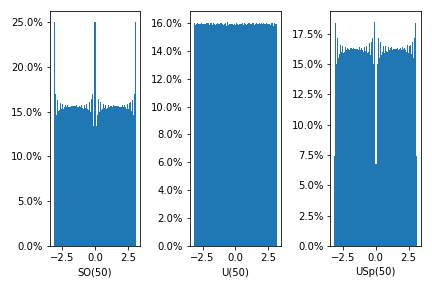
\includegraphics[width=.5\textwidth]{images/distributions.png}
\caption{Density plots of 100,000 $50\times 50$ matrices in (from the left) the special orthogonal group, the unitary and the unitary sympletic group.}\label{fig:densities}
\end{figure}


\subsubsection{Matrix sizes and cutoffs}

In order to compare the distributions of eigenvalues of random matrices and the low-lying zeros of L-functions, we have to determine the size of the matrices we use.  In this paper we study two different approaches to computing the matrix size and for each approach, we also determine the corresponding cutoff for the excised model.  See \cite{bm} for more details but we present the necessary results here.

The standard approach to finding the matrix size is to choose the matrix size $N_\std$ so that to choose that the mean densities of eigenvalues are equal to mean density of zeros.  In particular, this means that for discriminants around $X$ is $N_\std = \log\left ( \frac{\sqrt{3}X}{2\pi e}\right)$.  We point out that when we are modeling families using $SO(2N)$ or $USp(2N)$, we double $N_\std$.  When we model twists that correspond to the orthogonal group, we also use an effective matrix size that tries to capture the lower order terms in these densities.  In particular, there is a constant $a_1$ (defined below), such that the $N_\eff = \tfrac{N_\std}{2a_1}$.

For the orthogonal group, we also analyze a model (first described in \cite{DHKMS}) of low-lying zeros of twists of L-functions that incorporates the discretization that comes from Waldspurger's theorem.  In particular, for a modular form of weight $k$, the zeros are discretized by $1/D^{(k-1)/2}$ and so we exclude from our random matrices whose value at 1 is of the scale $\exp((1-k)N_\std/2)$; that is, we want matrices in $SO(2N)$
\[
\abs{\Lambda_A(1,N)} \geq c_\std\cdot \exp((1-k)N_\std/2)
\]
for some constant $c_\std$.  The effective cutoff $c_\eff$ is defined similarly except we replace the $\std$ subscripts with $\eff$.  

In \cite{DHKMS} and \cite{bm} formulas are given for these cutoffs, but we follow the numerical method to estimate the cutoffs described in \cite{DHKMS}.  In this approach they try several values of $c_\std$ (respectively $c_\eff$) and empirically measure the distance between the cumulative distributions of zeros (these are independent of the choice of cutoff) and eigenvalues (these will be greater than or equal to the cutoff) by numerically approximating the area between then at several specified points.  The value of $c_\std$ for which this is smallest, is the value we use.  In \cite{DHKMS}, the value of $c_\std$ for quadratic twists of the L-function associated to the modular form \texttt{11.2.a.a} was computed to be $\approx 2.188$ and this was shown to agree with the formula for $c_\std$ in the same paper.  We follow their approach and get a different value of $c_\std$\footnote{Their numerical value of $c_\std$ might be wrong because the mean value of the first zero that they report is incorrect as verified by our code, by Rubinstein's lcalc \cite{lcalc} and PARI/GP \cite{pari}}.

the zero distribution by averaging the
absolute value of the difference between the cumulative distribution of the zeros
and the cumulative distribution of the eigenvalues at a set of evenly spaced points

 
\subsection{Modular forms}

In what follows, we will consider L-functions attached to three different kinds of modular forms.  Let $f(q) = \sum_{n=1}^\infty a_nq^n \in S_k(M, \chi)$ be a newform of weight $k$, level $M$, and character $\chi$. Then three cases emerge:  \begin{enumerate}
\item\label{mf:regular} $f$ could have principal character, 
\item\label{mf:nsd} $f$ could have non-trivial character $(f\neq \overline{f})$, or
\item\label{mf:sd} $f$ could have complex multiplication by its own non-trivial character $(f=\overline{f})$.  
\end{enumerate}
In the above list, according to \cite{bm}, forms of type~\ref{mf:regular} should have L-functions whose quadratic twists have zeros that are modeled by random matrices from the orthogonal group, forms of type~\ref{mf:nsd} should have $L$-functions whose zeros are modeled by matrices from the unitary group and forms of type~\ref{mf:sd} should have $L$-functions whose zeros are modeled by matrices from the symplectic group.  

A newform is self-dual if its Fourier coefficients are real. A newform has complex multiplication (i.e., is CM) if there is a nontrivial Dirichlet character $\eta$ such that $\eta(p)a(p) = a (p)$ for all primes $p$ in a set of primes of density 1.  A form that is self-CM (as defined in \cite{bm}) is a form that is both self-dual and CM.


In order to make things more concrete, the particular modular forms we will consider are listed in Table~\ref{tbl:mfs}.

\begin{table}\small
\begin{tabular}{l|rr}
LMFDB label & Fourier expansion & Matrix group\\\hline\hline
\texttt{11.2.a.a} & $f(q)=  q - 2q^{2} - q^{3} + O(q^{4})$ & $\chi$ principal\\
\texttt{7.4.a.a} & $f(q)=q - q^{2} - 2q^{3} + O(q^{4})$ & $\chi$ principal\\
\texttt{3.6.a.a} & $f(q)=q - 6q^{2} + 9q^{3} + O(q^{4})$ & $\chi$ principal\\
\texttt{3.8.a.a} & $f(q) = q + 6q^{2} - 27q^{3} + O(q^{4})$ & $\chi$ principal\\
\texttt{3.10.a.b} & $f(q) = q + 18 q^{2} + 81 q^{3} + O(q^{4}) $ & $\chi$ principal \\\hline\hline
\texttt{13.2.e.a} & $f(q)= q + ( -1 - \zeta_{6} ) q^{2} + ( -2 + 2 \zeta_{6} ) q^{3} + O(q^{4})$ & $f\neq \overline{f}$\\\hline\hline
\texttt{7.3.b.a} & $f(q)= q - 3q^{2} + O(q^{4})$ & self-CM\\\hline\hline
\end{tabular}
\caption{Particular modular forms we will be using our experiments.  Here $\zeta_6$ is a particular $6$th root of unity.}\label{tbl:mfs}
\end{table}

\subsection{Admissible discriminants and families of L-functions}

Using the notation and terminology from above, we can now define the families of twists we will computing and comparing to the predictions from random matrix theory.

\begin{defn}\label{def:D}
  Let $\mathcal D$ denote the set of fundamental discriminants.  Let $f\in S_k(M,\chi_f)$ be a newform, with $M$ an odd prime. If $f$ is self-CM, assume $\ep_f=+1$.  With these restrictions on $f$, let $\heartsuit\in\{\pm1\}$ and $1\leq\diamondsuit<M$ be integers, and put
  \be\label{eq:dgooddef}\D(X):=\left\{\begin{aligned}
      &\left\{d\in\mathcal D:0<d\leq X\text{ and }\psi_d(M)\ep_f=+1\right\}
      &&\text{$\chi_f$ principal,} \\
      &\left\{d\in\mathcal D:0<d\leq X\text{ and }\psi_d(M)=\heartsuit \right\}
      &&\text{$f$ self-CM,} \\
      &\left\{d\in\mathcal D:0<d\leq X\text{ and }d\equiv\diamondsuit\mod M \right\}
      &&\text{$f\ne\overline f$.}\end{aligned}\right.\ee
\end{defn}
We now make precise our family $\F$.
\begin{defn}\label{def:F}
  Let \be\F(X):=\left\{L(f,s,\psi_D):d\in\D(X)\right\},\ee
  with $f\in S^k(M,\chi_f)$ be as in Definition~\ref{def:D}.
\end{defn}
Then, if $\chi_f$ is principal, $\F$ is the family of even quadratic twists of $L_f(s)$. If $f$ is self-CM, $\F$ is the subfamily of the family of even quadratic twists, with an added condition on the residue class of $d\mod M$.  If $f\ne\overline f$, then there is no notion of the parity of the functional equation of $L_f(s)$, and $\F$ is a subfamily of the family of quadratic twists of $L_f(s)$, with an added condition on the residue class of $d\mod M$.

\subsection{Computing central values modeled by orthogonal matrices}

To test some of the conjectures in this paper, we need to numerically compute the distribution of the central values of the families of quadratic twists described in Table~\ref{tbl:mfs}.  We now describe how we do this in the cases when the familiy of quadratic twists has central values modeled by orthogonal matrices.  In order to calculate these central values for modular forms with principal character we use standard approaches but carry them out for a wider range of weights and to higher discriminant bounds. 

\subsubsection{Weight 2}  For the modular form $f\in S_2(11)$ with label \texttt{11.2.a.a}, we follow the method described in \cite{MRVT} to compute central values $L(f,1/2,\psi_D)$, using Brandt matrices.

\subsubsection{Weight 4}
The first extensive computations of the modular form $f\in S_4(7)$ with label \texttt{7.4.a.a} and its Shimura lift were carried out in \cite{TR}.   We proceed in a similar way (the details are slightly different to be consistent with our other computations) and compute its Fourier expansion as
\[f = \frac{1}{4}\sum_{(a, b, c, d)\in\Z^4}(2a^2+2ab-3b^2)q^{Q_7(a, b, c, d)}\]
where $Q_7(a, b, c, d) = a^2 + ab +2b^2 + c^2 + bc + 2d^2 = Q_7'(a, b) + Q_7'(c, d)$, with $Q_7'(x, y) = x^2 + xy + 2y^2$.
Then
\[f = \frac{1}{4}\left(\sum_{(a, b)\in\Z^2}(2a^2+2ab-3b^2)q^{Q'_7(a, b)}\right)\left(\sum_{(b, c)\in\Z^2}q^{Q'_7(b, c)}\right),\]
and we can compute de Fourier coefficients of $f$ in linear time.

To compute the half integral modular form associated to $f$, $g_+$ we define
\[
w_{11}(x, y, z) = \left\{
\begin{array}{ll}
0&\text{if }11\nmid Q(x, y, z)\\
\left(\frac{-2x+z}{11}\right)&\text{if }2x\not\equiv z\pmod{11}\\
\left(\frac{x}{11}\right)&\text{otherwise}
\end{array}
\right.,
\]
and
\[g_+ = \frac{1}{4}\sum_{(x, y, z)\in\Z^3}xw_{11}(x, y, z)q^{Q(x, y, z)/11}=\sum_{n=1}^\infty c_+(n)q^n,\]
where $Q(x, y, z) = 4x^2+4xy+8y^2+7z^2$.
As before, we can compute this in linear time, this is because $xw_{11}(x, y, z)$ only depends on the variables $x$ and $y$,
and $Q(x, y, z) = Q'(x, y) + 7z^2$, where $Q'(x, y) = 4x^2+4xy+8y^2$.
So,
we define
\[
\sum_{n=1}^\infty a_n q^n = \frac{1}{4}\left(\sum_{(x, y)\in\Z^2}xw_{11}(x, y, 0)q^{Q'(x, y)}\right)\left(\sum_{z\in\Z}q^{7z^2}\right),
\]
so that
$c_+(n) = a_{11n}$.

\subsubsection{Weight 6}
For the modular form $f\in S_6(3)$ with label \texttt{3.6.a.a} we can compute its Fourier expansion as
\[f = \frac{1}{6}\sum_{(a, b, c, d)\in\Z^4}P(a, b, c, d)q^{Q_3(a, b, c, d)}\]
where $Q_3(a, b, c, d) = a^2 - ab + b^2 + c^2 - cd + d^2 = Q'_3(a, b) + Q'_3(a, b)$, $Q'_3(x, y) = x^2 - xy + y^2$, 
and $P(a, b, c, d) = a^4 - 2a^2c^2 - 2a^3b + 4ac^2b + 3a^2b^2 - 4b^2c^2 - 2ab^3 + b^4 - 2abcd + 4cb^2d - 2b^2d^2$.
So
\begin{align*}
f &= \\
\frac{1}{6}&\left(\sum_{(a, b)\in\Z^2}(a^4-2a^3b+3a^2b^2-2ab^3+b^4)q^{Q'_3(a, b)}\right)\left(\sum_{(c, d)\in\Z^2}q^{Q'_3(b, c)}\right)\\
+&\left(\sum_{(a, b)\in\Z^2}(-2a^2+4ab-4b^2)q^{Q'_3(a, b)}\right)\left(\sum_{(c, d)\in\Z^2}c^2q^{Q'_3(c, d)}\right)\\
-&\left(\sum_{(a, b)\in\Z^2}ab\,q^{Q'_3(a, b)}\right)\left(\sum_{(c, d)\in\Z^2}cd\,q^{Q'_3(c, d)}\right)\\
-&\left(\sum_{(a, b)\in\Z^2}2b^2\,q^{Q'_3(a, b)}\right)\left(\sum_{(c, d)\in\Z^2}d^2\,q^{Q'_3(b, c)}\right)\\
=&\left(\sum_{(a, b)\in\Z^2}(a^4-2a^3b+3a^2b^2-2ab^3+b^4)q^{Q'_3(a, b)}\right)\left(\sum_{(c, d)\in\Z^2}q^{Q'_3(b, c)}\right)\\
-&2\left(2\left(\sum_{(a, b)\in\Z^2}a^2q^{Q'_3(a, b)}\right)-\left(\sum_{(c, d)\in\Z^2}cd\,q^{Q'_3(c, d)}\right)\right)^2
\end{align*}

To compute the half integral modular form associated to $f$, $g_+$ we define
$Q_3(x, y, z) = 4x^2+4xy+4y^2 + 3z^2$,
\[
w_{7}(x, y, z) = \left\{
\begin{array}{ll}
0&\text{if }7\nmid Q_3(x, y, z)\\
\left(\frac{4x+5y}{7}\right)&\text{if }4x\not\equiv 5y\pmod{7}\\
\left(\frac{2x}{7}\right)&\text{otherwise}
\end{array}
\right.,
\]
\[
w_3(x, y, z) = \left(\frac{2x+y}{3}\right),
\]
and
\[
P(x, y, z) = 2x^2+2xy+2y^2-3z^2.
\]
Then
\[
g_+ = \frac{1}{6}\sum_{(x, y, z)\in\Z^3}P(x, y, z)w_3(x, y, z)w_7(x, y, z)q^{Q_3(x, y, z)}.
\]
Because $w_3$ and $w_7$ only depends in the variables $x, y$ we can compute the coefficients
of $g_+$ in linear time as before.

\subsubsection{Weight 8}
For the modular form $f\in S_8(3)$ with label \texttt{3.8.a.a} we can compute its Fourier expansion as
\[f = \frac{1}{6}\sum_{(a, b, c, d)\in\Z^4}P(a, b, c, d)q^{Q_3(a, b, c, d)}\]
with $Q_3$ as before, and
$P(a, b, c, d) = 2a^{6} - 6a^{5} b - 15a^{4} b^{2} + 40a^{3} b^{3} - 15a^{2} b^{4} - 6a b^{5} + 2b^{6} + 2c^{6} - 6c^{5} d - 15c^{4} d^{2} + 40c^{3} d^{3} - 15c^{2} d^{4} - 6c d^{5} + 2d^{6}
= P_1(a, b) + P_1(c, d)$.
So,
\[
f = \frac{1}{6}\left(\sum_{(a, b) \in\Z^2}P_1(a, b)q^{Q'_3(a, b)}
\right)
\sum_{(c, d)\in\Z^2}q^{Q'_3(c, d)}
.\]

To compute the half integral modular forma associated to $f$, $g_+$ we define
$P(x, y, z) = 2x^3 + 3x^2y - 3xy^2 - 2y^3$,
and we have
\[
g_+ = \frac{1}{6}\sum_{(x, y, z)\in\Z^3}P(x, y, z)w_7(x, y, z)q^{Q_3(x, y, z)},
\]
and as before we can compute the coefficients of $g_+$ in linear time.

\subsubsection{Weight 10}
For the modular form $f\in S_8(3)$ with label \texttt{3.10.a.b} we can compute its Fourier expansion as
\[f = \frac{1}{6}\sum_{(a, b, c, d)\in\Z^4}P(a, b, c, d)q^{Q_3(a, b, c, d)}\]
with $Q_3$ as before, and
\begin{align*}
P(a, b, c, d) &= a^8 - 4a^7b + 10a^6b^2 - 16a^5b^3 + 19a^4b^4 - 16a^3b^5 + 10a^2b^6\\
& - 4ab^7 + b^8 - 16a^6c^2 + 48a^5bc^2 - 96a^4b^2c^2 + 112a^3b^3c^2 - 96a^2b^4c^2 \\
& + 48ab^5c^2 - 16b^6c^2 + 36a^4c^4 - 72a^3bc^4 + 108a^2b^2c^4 - 72ab^3c^4 + 36b^4c^4\\
& - 16a^2c^6 + 16abc^6 - 16b^2c^6 + c^8 + 16a^6cd - 48a^5bcd + 96a^4b^2cd  \\
& -112a^3b^3cd + 96a^2b^4cd - 48ab^5cd + 16b^6cd - 72a^4c^3d + 144a^3bc^3d - 216a^2b^2c^3d\\
& + 144ab^3c^3d - 72b^4c^3d + 48a^2c^5d - 48abc^5d + 48b^2c^5d - 4c^7d - 16a^6d^2\\
& + 48a^5bd^2 - 96a^4b^2d^2 + 112a^3b^3d^2 - 96a^2b^4d^2 + 48ab^5d^2 - 16b^6d^2 + 108a^4c^2d^2\\
& - 216a^3bc^2d^2 + 324a^2b^2c^2d^2 - 216ab^3c^2d^2 + 108b^4c^2d^2 - 96a^2c^4d^2 + 96abc^4d^2 - 96b^2c^4d^2\\
& + 10c^6d^2 - 72a^4cd^3 + 144a^3bcd^3 - 216a^2b^2cd^3 + 144ab^3cd^3 - 72b^4cd^3 + 112a^2c^3d^3 \\
&- 112abc^3d^3 + 112b^2c^3d^3 - 16c^5d^3 + 36a^4d^4 - 72a^3bd^4 + 108a^2b^2d^4 - 72ab^3d^4\\
&+ 36b^4d^4 - 96a^2c^2d^4 + 96abc^2d^4 - 96b^2c^2d^4 + 19c^4d^4 + 48a^2cd^5 - 48abcd^5\\
& + 48b^2cd^5 - 16c^3d^5 - 16a^2d^6 + 16abd^6 - 16b^2d^6 + 10c^2d^6 - 4cd^7 + d^8.
\end{align*}

To compute the half integral modular form associated to $f$, $g_+$ we define
$P(x, y, z) = 2x^4+4x^3y+6x^2y^2+4xy^3+4xy^3+2y^4+2y^4-12x^2z^2-12xyz^2-12y^2z^2+3z^4$,
and we have
\[
g_+ = \frac{1}{6}\sum_{(x, y, z)\in\Z^3}P(x, y, z)w_3(x, y, z)w_7(x, y, z)q^{Q_3(x, y, z)},
\]
and as before we can compute the coefficients of $g_+$ in linear time.

\subsection{Computing central values modeled by symplectic and orthogonal matrices}

In contrast with families of quadratic twists of modular forms with principal character, if the modular form being twisted has nonprincipal character, the situation is quite different.  First, as there is no analogue of Waldspurger's Theorem or the explicit constructions of Gross--Kohnen--Zagier, we are left with computing the L-functions using the implementations available in PARI/GP \cite{pari} and described in \cite{paribook}.  These computations are based on the Booker-Molin idea for computing $\Lambda(s)$.  Since the difficulty of the computations grow quadratically with the conductor of the twist, our computations are much more limited.    

\subsection{Computing first few zeros of L-functions}

Our ultimate goal is to understand the distribution of zeros, we describe now how we calculate them.  Again, we use the implementation in PARI/GP \cite{pari} that is described in \cite{paribook}.  Roughly speaking, a naive search is done for zeros of the real-valued Hardy Z-function along the critical line $s=1/2$. The computations here are limited due to the complexity of calculating zeros of L-functions of large conductor.  In each case, we compute the first few zeros of twists of the curves in Table~\ref{tbl:mfs} up to discriminant 40,000. 





\section{Results}


\subsection{Distributions}  Recall that the three types of families that we are considering are those that can be modeled by $SO(2N)$, $U(N)$ and $USp(2N)$ and in each case we have zeros for twists up to discriminant 40,000.  In this first experiment, we compare the distributions of the eigenvalues and zeros, normalized so that they both have means of 1 and observe that the shape of each pair of plots in Figure~\ref{fig:dists} are similar.  In our computations of the eigenvalues, we calculated $N_\std$ for each discriminant $D$ and then found the mean lowest eigenvalue over a sample of $10,000$ matrices.
\begin{figure}
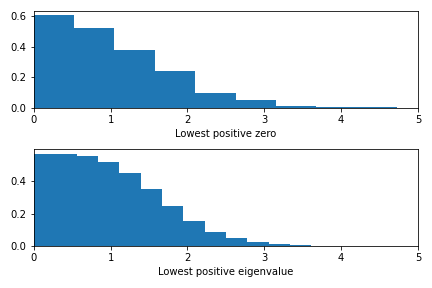
\includegraphics[width=.3\textwidth]{images/exp1.png}\hfill
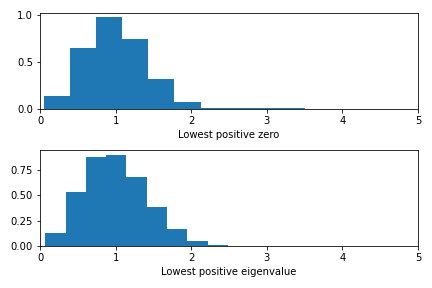
\includegraphics[width=.3\textwidth]{images/exp2.png}\hfill
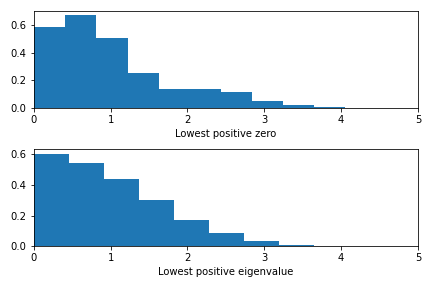
\includegraphics[width=.3\textwidth]{images/exp3.png}\\
\caption{Distributions of lowest zeros of admissible twists of \texttt{3.8.a.a} and lowest mean eigenvalues from $SO(2N)$ (left), distributions of lowest zeros of admissible twists of \texttt{13.2.e.a} and lowest mean eigenvalues from $USp(2N)$ (center), and distributions of lowest zeros of admissible twists of \texttt{7.3.b.a} and lowest mean eigenvalues from $U(N)$ (right). The data have been normalized to have a mean of one.}
\label{fig:dists}
\end{figure}


\subsection{Repulsion} Now, we verify the expectation that the average repulsion is less for larger conductors that it is for smaller conjectures. For each of these plots we broke the set of admissible twists, ordered by discriminant, in half and called the first half as being of ``small'' conductor and the second half as being of ``large'' conductor.  According to the philosophy of the correspondence between zeros of L-functions and random matrix theory, as the discriminant of the twist goes to infinity, the repulsion goes to zero since this corresponds to the matrix size tending to infinity, and hence the smallest eigenvalue tends to 1, corresponding to an angle of 0.  In Figure~\ref{fig:repulsion} we observe this phenomenon: as predicted by random matrix theory the repulsion (as measured by the mean of the lowest zeros in each group) decreases with larger discriminants.
\begin{figure}
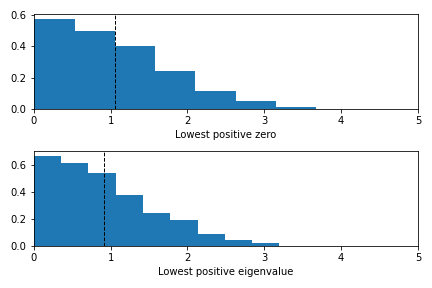
\includegraphics[width=.3\textwidth]{images/exp1-lo-hi.png}\hfill
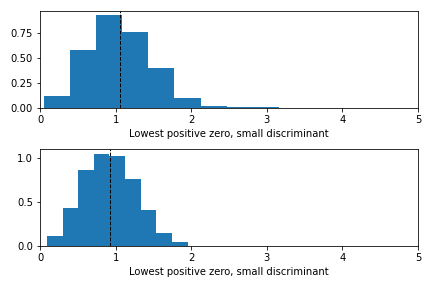
\includegraphics[width=.3\textwidth]{images/exp2-lo-hi.png}\hfill
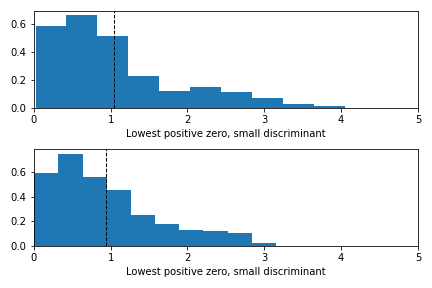
\includegraphics[width=.3\textwidth]{images/exp3-lo-hi.png}\\
\caption{Distributions of lowest zeros of admissible twists of \texttt{3.8.a.a} separated into those of small and large conductor (left), distributions of lowest zeros of admissible twists of \texttt{13.2.e.a} separated into those of small and large conductor (center), and distributions of lowest zeros of admissible twists of \texttt{7.3.b.a} separated into those of small and large conductor (right).  The dashed vertical lines in each graph are the means of the data; and, again, the data have been normalized to have a mean of one.}\label{fig:repulsion}
\end{figure}

\subsection{Cutoffs}  In this experiment we study how well the excised model does compared to the standard model that does not take intro account the discretization from Waldspurger's theorem.  In order to do this we first need to find the cutoffs for the forms we are considering; recall that because of the difficulty in computing central values of forms not modeled by the orthogonal group, we are limiting our attention to those forms for which $\psi$ is principal.

As described above, we numerically approximate the value of $c_\std$ by comparing, for various candidates of $c_\std$ the cumulative distributions of central values cut off at the candidate value of $c_\std$ and the cumulative ditribution of evaluations of characteristic polynomials at 1 cut off at the candidate value of $c_\std$.  We make a plot of these differences for each candidate value of $c_\std$ and find the minima on each plot.  As the weight increases, the computations of the central values get harder and so the plots are less smooth for larger weight.  See Figure~\ref{fig:c_std}.  

The value of $c_\std$ for twists of \texttt{11.2.a.a} was roughly $1.6$, the value of $c_\std$ for twists of \texttt{7.4.a.a} was roughly $26,500$, the value of $c_\std$ for twists of \texttt{3.6.a.a} was roughly $2.97\times 10^9$, and the value of $c_\std$ for \texttt{3.8.a.a} was roughly $7.08\times 10^{14}$.   

\begin{figure}
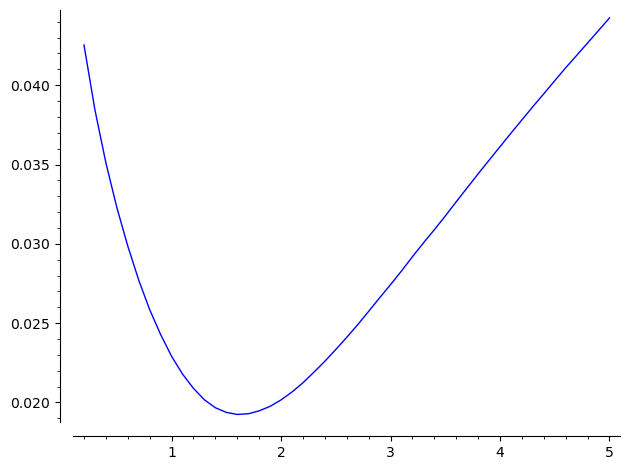
\includegraphics[width=.2\textwidth]{images/c_std-11-2.png}\hfill
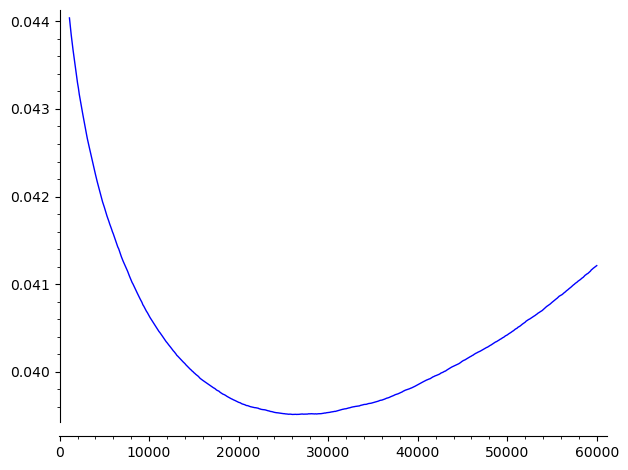
\includegraphics[width=.2\textwidth]{images/c_std-7-4.png}\hfill
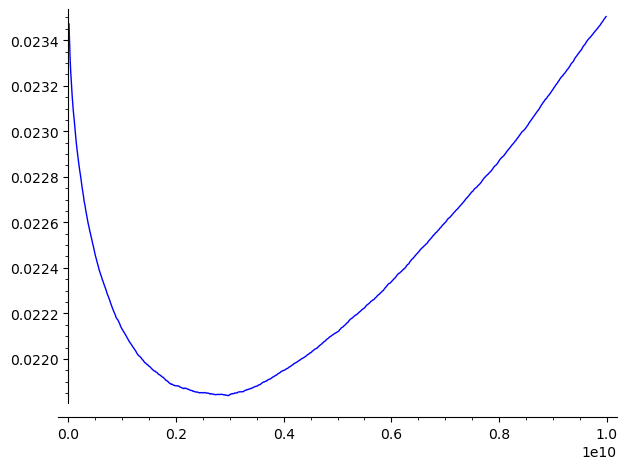
\includegraphics[width=.2\textwidth]{images/c_std-3-6.png}\hfill
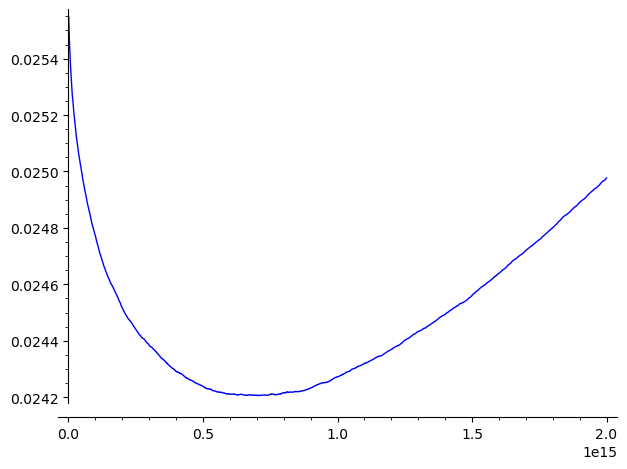
\includegraphics[width=.2\textwidth]{images/c_std-3-8.png}
\caption{Each of these four plots shows the difference, for various candidate values of the cutoff $c_\std$, between the cumulative distributions of values of $L(f,1/2,\psi_D)$ and of values of $\Lambda_A(1,N)$.  From left to right the forms whose central values $f$ are being calculated are \texttt{11.2.a.a}, \texttt{7.4.a.a}, \texttt{3.6.a.a}, and \texttt{3.8.a.a}.  From left to right the values of $N$ used were$\dots$}\label{fig:c_std}
\end{figure}



\subsection{Effective versus standard}









\bibliography{zeros} 
\bibliographystyle{plain}


\end{document}




Now we turn from the raw data associated to twists of these three types of L-functions and to the comparison of these data with the corresponding data from random matrix theory.  In this section we do not concern ourselves with excising the model, we pick that up in the next section.  The random matrices were computed in SageMath \cite{sage}, the zeros of the twists were computed in PARI/GP \cite{pari}, the histograms were made in Python.  The code and data are available at \cite{code}.

\subsection{Simple model}

Our first round of experiments were to verify two expectations.  First, we want to see that distributions of zeros of $L$-functions of each type (self-dual, non-self-dual and self-CM) roughly matched the distributions of eigenangles for the corresponding group of matrices.  Additionally, we illustrate that we get the expected decrease in repulsion as the discriminant of the twist increases.

\subsubsection{Trivial nebentypus}

Let $f\in S_k(M,\chi)$ be one of the four newforms in Table~\ref{tbl:mfs} with $\chi$ principal; let $\mathscr{D}_f (X )$ be as in Definition~\ref{def:D}. We calculate the distribution of the lowest zero for $L(f,s,\psi_D )$ for $d \in \mathscr{D}_f (X )$, provided $L(f,1/2, \psi_D ) \neq 0$. We also also calculate the distribution of the lowest eigenvalue for $\textrm{SO}(2N_{\text{std}} )$ where $N_\text{std}$ for discriminants around $X$ is given by 
\[
N_\text{std} = \log\left (\frac{\sqrt{M}X}{2\pi e}\right ).
\]
See Figure~\ref{fig:trivial-plots} for plots of the distributions of the zeros of the $L$-functions with the expected random matrix theory distribution overlaid. 

\ncr{Gustavo:  do you have easy access to make the data of these 5 plots?  Up tp what $X$?}

\subsubsection{Self-CM} 

Let $f$ be the self-CM form with LMFDB label \texttt{7.3.b.a}. Let $\mathscr{D}_f (X )$ be as in Definition~\ref{def:D} for $\chi_f$ non-trivial. We calculate the distribution of the lowest zero for $L(f,s,\psi_D )$ for $d \in \mathscr{D}_f (X )$, provided $L(f ,1/2, \psi_D ) \neq 0$. We also also calculate the distribution of the lowest eigenvalue for $\textrm{USp}(N_{\text{std}} )$ where $N_\text{std}$ for discriminants around $X\approx 40000$ is given by 
\[
N_\text{std} = \log\left (\frac{\sqrt{7}X}{2\pi e}\right ) = 8.73\dots.
\]
See Figure~\ref{fig:sd-plots} for plots that show both the expected decrease in repulsion as $D$ increases and that compare the distribution of the zeros with distribution of the eigenangles.

\begin{figure}  
%\includegraphics[width=.5\textwidth]{sd.png}\hfill \includegraphics[width=.5\textwidth]{sd-lo-hi.png}
\caption{The figure on the left is a comparison of the distributions of lowest psitive zeros for the form whose LMFDB label is \texttt{7.3.b.a} and the lowest positive eigenangle for $USp(8)$.  The data were normalized so that they would have the same mean and these plots were such that $\psi_D(7) = +1$.  The figure on the right is a comparison of the distributions for the lowest postive eigenangle for smaller and larger values of $D$.  Observe the expected reduction in repulsion with larger $D$. In both figures, the vertical dashed line indicates the mean of the distribution. }\label{fig:sd-plots}
\end{figure}



\subsubsection{Non self-dual} 

Let $f$ be the non self-dual form with LMFDB label \texttt{13.2.e.a}. Let $\mathscr{D}_f (X )$ be as in Definition~\ref{def:D} for $\chi_f$ non-trivial. We calculate the distribution of the lowest zero for $L(f,s, \psi_D )$ for $d \in \mathscr{D}_f (X )$, provided $L(f,1/2, \psi_D ) \neq 0$. We also also calculate the distribution of the lowest eigenvalue for $\textrm{U}(N_{\text{std}} )$ where $N_\text{std}$ for discriminants around $X\approx 40000$ is given by 
\[
N_\text{std} = \log\left (\frac{\sqrt{13}X}{2\pi e}\right ) = 9.04\dots
\]
See Figure~\ref{fig:nsd-plots} for plots that show both the expected decrease in repulsion as $D$ increases and that compare the distribution of the zeros with distribution of the eigenangles.

\begin{figure}  
%\includegraphics[width=.5\textwidth]{nsd.png}\hfill \includegraphics[width=.5\textwidth]{nsd-lo-hi.png}
\caption{The figure on the left is a comparison of the distributions of lowest psitive zeros for the form whose LMFDB label is \texttt{13.2.e.a} and the lowest positive eigenangle for $U(9)$.  The data were normalized so that they would have the same mean and these plots were such that $D \equiv 7 \pmod{13}$.  The figure on the right is a comparison of the distributions for the lowest postive eigenangle for smaller and larger values of $D$.  Observe the expected reduction in repulsion with larger $D$. In both figures, the vertical dashed line indicates the mean of the distribution.}\label{fig:nsd-plots}
\end{figure}

 



\subsection{Excising the model}

In this section we restrict to examples of $L$-functions for modular forms that are self-dual and have trivial character.  We do this because the other two kinds of modular forms we considered in the previous section do not really have a central value and, in particular, do not have a Waldspurger-type or Kohnen--Zagier-type formula.

As mentioned above,  by Waldspurger's theorem \cite{Waldspurger} and, more explicitly by the Kohnen--Zagier formula \cite{KZ} $L(f, 1/2, \psi_D)$ is discretized.  In particular, suppose a modular form of weight 2 corresponds to $h=\sum c(n)q^n$ in the Kohnen plus space of weight 3/2, with $c(n)\in\mathbb{Z}$.  Then,
\[
L(f,1/2,\psi_D) = \frac{\kappa_f c(\abs{d})^2}{\abs{d}^{1/2}},
\]
where $\kappa_f > 0$ depends only on $f$ and $g$ and not on $\psi_d$.  This means, for example, that if  $L(f,1/2,\psi_D) < \kappa_f \abs{d}^{-1/2}$ then it is equal to zero.  And, moreover, it means that for the L-funcitons in the families we are considering (they are rank 0), we know $L(f,1/2,\psi_D) > \kappa_f \abs{d}^{-1/2}$.  

In the previous sections, we freely sampled from the entire space of random matrices.  In this section we sample from a subspace.  In \cite{CF,CKRS,CKRS2,KS} it was shown that values of L-functions at the central point can be modeled using characteristic polynomials evaluated at the point 1.  So, in analogy with the values $L(f,s,\psi_D)$ is not allowed to take on, we model rank 0 curves by discarding from our sample space all random matrices $A$ whose characteristic polynomial $\Lambda_A(z,N)$ is away from 0 when evaluated at $z=1$.  

In \cite{bm}, it is shown that the cutoff will be of the form
\[
\abs{\Lambda_A(1,N)} \geq c_{\text{std}}\times\exp((1-k)N_{\text{std}}/2)
\]
and in this section we estimate the constant $c_{\text{std}}$ for the first three of the four modular forms with trivial character listed in Table~\ref{tbl:mfs}.

In this section we consider forms of weights 2, 4 and 6 and study how well the low-lying zeros of their associated L-functions are modelled using the excised model.  In particular, we approximate the choice of $c_\text{std}$.  See Table~\ref{tbl:triv-forms} for the forms that we use.

To find the value of $c_\text{std}$ numerically, we proceed as follows.  Let $f$ be the form we are considering and suppose it is of level $M$.  Calculate as many central values of $L(f,1/2,\psi_D)$ as possible (see Table~\ref{tbl:mfs}).  Let $N_\text{std}$ be the size of the group of random matrices used to model the zeros of $f$.  Let $c$ be a candidate value for $c_\text{std}$.  Then we calculate a sample of $10^{7}$ matrices $A$\ncr{is this right?} in $SO(2N_\text{std})$ such that $\Lambda_A(1,N_\std) \geq c \exp((1-k)N_\std/2)$.  Then for this $c$ we compare the distibution of zeros and eigenangles.  In particular, we measure the agreement between the distribution of the central values and the distribution of the characteristic polynomials evaluated at 1 (normalized to have the same mean) by averaging the absolute value of the difference between the cumulative distribution of the zeros and the cumulative distribution of the eigenvalues at a set of evenly spaced points.\ncr{Gustavo:  is this right?}  See Figure~\ref{fig:numerical-c} for three such plots.  See Table~\ref{tbl:results} for a summary of our results.


\subsubsection{Calculations}



\subsubsection{Results}

\begin{figure}
\centering
%\includegraphics[width=.3\textwidth]{112.png} \hfill \includegraphics[width=.3\textwidth]{74.png} \hfill \includegraphics[width=.3\textwidth]{36.png}
\caption{A measure of the difference between the mean-scaled cumulative distribution of the first eigenangle of the excised random with $N_\std = 12$ for various candidates $c$ for $c_\std$ and the cumulative distribution of the first zero of even quadratic twists $L(f,s,\psi_D)$ with $D$ as in Definition~\ref{def:D} and for $f$ of weights 2, 4 and 6 from left to right.  Their respective minima are at XXX.}\label{fig:numerical-c}
\end{figure}


\begin{table}[h]
\centering
\begin{tabular}{l|rrrrrr}
Weight & Label & $f$ & $g$ & $\kappa_f$ & \# coeffs & $\mathscr{L}_M(X,f)$\\\hline
4 & & & & & \\
6 & & & & &\\
8 & & & & &\\
10 & & & & &\\\hline
\end{tabular}
\caption{A table of the forms $f$ for which we calculate $c_\text{std}$.  We report the form's LMFDB label, the first few coefficients of $f$, the first few coefficients of the Shimura lift $g$ of $f$, the constant $\kappa_f$ in the Kohnen-Zagier formula and the number of coefficients we can calculate for $g$.  We also report the local factor of the L-function at $M$, the level of $f$.}\label{tbl:triv-forms}
\end{table}


\begin{table}
\centering
\begin{tabular}{l|rrrrrr}
Label & $a_f(1/2)$ & $\delta_f$ & $N_\text{std}$ & \# matrices & $c_\text{std}$ approx & $c_\text{std}$ formula \\\hline
 & & & & & &\\
 & & & & & &\\
 & & & & & &\\
 & & & & & &\\\hline
\end{tabular}
\caption{A table of results, intermediate and final, related to find $c_\text{std}$ for the $f$ in Table~\ref{tbl:forms}.  }\label{tbl:results}
\end{table}

\subsubsection{Verification}

In \cite{bm} and \cite{DHKMS}, a formula is given calculate $c_\std$ in terms of 

As further confirmation, we compute $c_\text{std}$ using the following formula:
\[
c_\text{std} \times \exp((1-k)N_\text{std}/2) := a_f^{-2}(-1/2)\delta_f \kappa_f \times \exp((1-k)N_\text{std}/2)
\]
where $\kappa_f$ is the constant in the Kohnen-Zagier formula, 
\begin{multline*}
a_f(m) = \left [\prod_p \left ( 1-\tfrac{1}{p}\right )^{m(m-1)/2}\right ] \\
\times \left [ \prod_{p \nmid M} \left( 1+\tfrac{1}{p}\right )^{-1}\left(\tfrac{1}{p} + \tfrac{1}{2}\left [ \mathscr{L}_p(p^{-1/2},f)^m + \mathscr{L}_p(-p^{-1/2},f)^m\right ] \right ) \right] \\
\times \mathscr{L}_M\left (\tfrac{\epsilon_f}{M^{1/2}},f\right )^m 
\end{multline*}
and 
\[
\sqrt{\delta_f} = \frac{\abs{\{ L(f,s,\psi_D)\in \mathscr{F}_f: d\text{ prime}, L(f,1/2,\psi_D)=0\}}}{\sum^*_{d\text{ prime}} 2a_f(-1/2)\sqrt{\kappa_f}d^{(1-k)/4} h(\log d)}.  
\]
Here \ncr{eigenvalues are normalized by dividing by $p^{(k-1)/2}$}\ncr{in the paper there is a $+$ superscript on $\mathscr{D}$ and $\mathscr{F}$ sometimes}\ncr{I think $\chi_f(p)=1/p$}
\begin{align*}
\mathscr{L}_p(X,f) &= (1-\lambda_f(p)X+\chi_f(p)X^2)^{-1} \\
\mathscr{F}_f(X) &= \{L(f, s, \psi_D): d\in \mathscr{D}_f(X)\}\\
\mathscr{D}_f(X) &= \{d \text{ fundamental}: 0<d \leq X\text{ and }\psi_d(M)\epsilon_f=+1\}\\
\mathscr{F}_f &= \lim_{X\to\infty} \mathscr{F}_f(X)\\
\sum^* &=  \text{ sum $d$ fundamental, prime such that $L(f,s, \psi_D)$ has an even functional equation},\\
h(N) &= 2^{-N}\Gamma(N)^{-1} \prod{j=1}^N \frac{\Gamma(N+j-1)\Gamma(j)}{\Gamma(j-1/2)\Gamma(j+N-3/2)}.
\end{align*}
 

